\documentclass[useAMS,usenatbib,referee]{biom}

\usepackage{amsmath}
\usepackage[figuresright]{rotating}

\graphicspath{{../temp/rna-seq-stan/fig-rm-stan_laplace/}}

%%%%% PLACE YOUR OWN MACROS HERE %%%%%

\def\bSig\mathbf{\Sigma}
\newcommand{\VS}{V\&S}
\newcommand{\tr}{\mbox{tr}}

\title{Empirical Bayes analysis for detection of gene heterosis in RNAseq data}

\author{Jarad Niemi$^*$\email{niemi@iastate.edu}, 
Eric Mittman, 
Will Landau, and 
Dan Nettleton \\
Department of Statistics, Iowa State University, Ames, Iowa, U.S.A.}

\begin{document}

\date{{\it Received December} 2014} 

\pagerange{\pageref{firstpage}--\pageref{lastpage}} 
\volume{VV}
\pubyear{YYYY}
\artmonth{Month}
\doi{x}

\label{firstpage}

%  put the summary for your paper here

\begin{abstract}
This is the summary for this paper.
\end{abstract}

\begin{keywords}
Empirical Bayes; Heterosis; Hierarchical Model; Negative binomial; RNAseq.
\end{keywords}

\maketitle

%  A maximum of six (6) tables or figures combined is often required.''

\section{Introduction}
\label{s:intro}

\section{Heterosis}
\label{s:heterosis}

Well before heterosis was scientifically described by \cite{darwin1876effects}, humans had been using heterosis for various practical purposes. Within the last century, heterosis has been used to improve many species for food, feed, and fuel industries. A few relatively recent examples include rice \cite{yu1997importance}, alfalfa \cite{riday2002heterosis}, tomatoes \cite{krieger2010flowering}, and fish \cite{wohlfarth1993heterosis}. Despite the intensive study and successful utilization of heterosis, the basic genomic mechanisms responsible for heterosis remain unclear \cite{lippman2007heterosis}.

\cite{shull1952beginnings} coined the term heterosis and defined it as 
\begin{quote}
the interpretation of increased vigor, size, fruitfulness, speed of development, resistance to disease and to insect pests, or to climatic rigors of any kind, manifested by crossbred organisms as compared with corresponding inbreds, as the specific results of unlikeness in the constitutions of the uniting parental gametes.
\end{quote}

For example, the maize hybrid produced from a cross of parental inbred lines B73 and Mo17 is larger in size, has lower maturation time, and has higher grain yield than both of its parents \cite{hallauer2010quantitative}. Data from \citep{paschold2012complementation}

\citep{ji2014estimation}


\section{Empirical Bayes identification of gene heterosis from RNAseq counts}

To identify genes displaying heterosis using RNAseq data, we build a hierarchical model to borrow information on gene-variety means as well as overdispersion parameters, estimate the parameters using a empirical Bayes procedure implemented in the statistical software {\tt Stan}, and calculate posterior probabilities for heterosis. 

\subsection{Hierarchical model for RNAseq counts}
\label{s:model}

Let $Y_{gvi}$ be the count for gene $g=1,\ldots,F$, variety $v=1,\ldots,V$, and replicate $i=1,\ldots,n_v$. As shown in equation \eqref{e:data}, we assume a negative binomial for the counts with a mean that depends on the gene-variety combination through $\mu_{gv}$ and the sequencing depth $c_{vi}$ and a gene-specific over-dispersion $\psi_g$. Here $NB(\eta,\psi)$ indicates a negative-binomial with expectation $\eta$ and variance $\eta+\psi\eta^2$ and $ind$ indicates the observations are conditionally independent.
\begin{equation} 
Y_{gvi} \stackrel{ind}{\sim} NB(e^{\mu_{gv}+\delta_{vi}},\psi_g) 
\label{e:data}
\end{equation}

A hierarchical model is constructed for the sequencing depth, overdispersion, and gene-variety parameters. The sample-specific sequencing depth terms are assumed to follow a normal distribution, i.e. $\delta_{vi} \stackrel{ind}{\sim} N(0,\tau_\delta^2)$. The logarithm of the gene-specific over-dispersion parameters also follow a normal distribution $\log(\psi_g) \stackrel{ind}{\sim} N(\zeta_\psi,\tau_\psi^2)$. The variety-specific effects for each gene, $\mu_g = (\mu_{g1},\ldots,\mu_{gV})'$ are assumed to have a joint normal distribution $\mu_g \stackrel{ind}{\sim} N(\eta, \Sigma)$. We consider an \emph{independent} model where $\Sigma$ is diagonal with elements $\sigma_1^2,\ldots,\sigma_V^2$ and a \emph{covariance} model where we estimate all parameters in $\Sigma$. 

We assume improper uniform priors for all hierarchical means and half-Cauchy priors for standard deviations \citep{gelman2006prior}, e.g. $\tau_\delta, \tau_\psi \stackrel{ind}{\sim} Ca^+(0,3)$ where 0 and 3 are the location and scale parameters of the untruncated distribution. In the independent model, we also assume $Ca^+(0,3)$ on the diagonal elements while in the covariance model, we assume a conjugate, proper inverse Wishart with degrees of freedom $V+1$ and an identity scale matrix. 

\subsection{Empirical Bayes}
\label{s:ebayes}

The parameters from the model in Section \ref{s:model} can be group by gene-specific parameters $\theta_g = (\mu_g,\psi_g)$, collectively $\theta = (\theta_1,\ldots,\theta_G)$, and hyperparameter $\phi = (\delta, \zeta_\psi, \tau_\psi^2, \Sigma)$ where $\delta = (\delta_{11},\ldots,\delta_{Vn_V})$. We employ an optimization procedure to obtain the \emph{maximum a posteriori} (MAP) estimate for $\phi$ and then base gene-specific inference on the posterior conditional on this estimated hyperparameter. Conditional on the hyperparameters, the gene specific parameters are conditionally independent as in equation \eqref{e:condind}. 
\begin{equation}
p(\theta|y,\hat{\phi}_{MAP}) = \prod_{g=1}^G p(\theta_g|y_g,\hat{\phi}_{MAP}) \propto \prod_{g=1}^G NB(y_g|\theta_g,\hat{\delta}_{MAP})N(\theta_g|\hat{\mu}_{MAP}, \hat{Sigma}_{MAP}) 
\label{e:condind}
\end{equation}
Thus, conditional posterior inference for the gene specific parameters can be obtained independently and in parallel.

To perform the optimization, we use the statistical software {\tt Stan} \citep{stan-software:2014} run through the RStan interface \citep{rstan-software:2014} in R \citep{R2014}. The Stan software allows construction of general Bayesian models with the primary restriction that all unknown parameters must be continuous. Once a model is constructed, the software can be used to obtain MAP estimates \cite[see Section 50.3]{stan-manual:2014} using the {\tt optimizing} function in RStan. We found it necessary to use the L-BFGS algorithm \cite[see Section 55]{stan-manual:2014}. Alternatively, the software can be used to run a Markov chain Monte Carlo (MCMC) algorithm to obtain samples from the posterior using the {\tt sampling} function in RStan. By default, Stan uses a variant of Hamiltonion Monte Carlo \citep{neal2011mcmc} called the No-U-turn sampler \citep{hoffman2013no}. 

As we have not integrated out the gene-specific parameters when obtaining the MAP estimate, we actually receive a joint MAP estimate for $\theta$ and $\phi$. We explicitly use the MAP estimate for $\phi$ when obtaining empirical Bayes posterior samples for the gene specific parameters. The MAP estimate for $\theta$ can also be used in this step as initial values for the MCMC. 

\subsection{Gene heterosis}
\label{s:gene_heterosis}

As defined in Section \ref{s:heterosis}, heterosis is increased (or decreased) phenotypic expression in a hybrid relative to its inbred parents. Thus, when attempting to identify heterosis, there are three varieties of interest, i.e. $V=3$. We let $v=1,2$ be the two parental varieties and $v=3$ be the hybrid. We define gene heterosis to be the differential expression of the hybrid relative to its parents. For a specific gene $g$, low-parent gene heteorisis (LPH) occurs when $\mu_{g3}< \min(\mu_{g1},\mu_{g2})$, mid-parent gene heterosis occurs when $\mu_{g1}\le \mu_{g3}\le \mu_{g2}$ if $\mu_{g1}\le \mu_{g2}$ (or $\mu_{g1}\ge \mu_{g3}\ge \mu_{g2}$ if $\mu_{g1}\ge \mu_{g2}$), and high-parent gene heterosis (HPH) occurs when $\max(\mu_{g1},\mu_{g2}) < \mu_{g3}$. For simplicity, we define \emph{extreme gene heterosis} (EH) which is the event LPH or HPH. Of interest is to evaluate the hypotheses shown in equation \eqref{e:hypotheses} where $H_0$ indicates no EH and $H_1$ indicates EH. 
\begin{align}
\label{e:hypotheses}
H_{g0}:&\mu_{g1}\le \mu_{g3}\le \mu_{g2} \mbox{ or } \mu_{g1}\ge \mu_{g3}\ge \mu_{g2} \mbox{\ \ vs.\ \ } \nonumber \\
H_{g1}:&\mu_{g3}< \min(\mu_{g1},\mu_{g2}) \mbox{ or } \max(\mu_{g1},\mu_{g2}) < \mu_{g3}.
\end{align}
We evaluate these hypotheses based on empirical Bayes estimates of their posterior probability, e.g. 
\begin{align}
P\left(H_{g1}|y, \hat{\phi}_{MAP}\right) &= P\left(\left.\mu_{g3}< \min(\mu_{g1},\mu_{g2}) \mbox{ or } \max(\mu_{g1},\mu_{g2}) < \mu_{g3}\right| y, \hat{\phi}_{MAP}\right) \nonumber \\
&\approx \frac{1}{M} \sum_{m=1}^M \mathrm{I}\left(\mu_{g3}^{(m)}< \min\left(\mu_{g1}^{(m)},\mu_{g2}^{(m)}\right) \mbox{ or } \max\left(\mu_{g1}^{(m)},\mu_{g2}^{(m)}\right) < \mu_{g3}^{(m)}\right) \label{e:probs}
\end{align}
where $\mu_g^{(m)} = \left(\mu_{g1}^{(m)},\mu_{g2}^{(m)},\mu_{g3}^{(m)}\right)$ is the $m^{th}$ MCMC sample from the empirical Bayes posterior and $\mathrm{I}(A)$ is 1 if A is true and 0 otherwise. The set of probabilities $P\left(H_{g1}|y, \hat{\phi}_{MAP}\right)$ for $g=1,\ldots,G$ can be used to provide a sorted list of genes potentially involved in phenotypic heterosis. 

\section{Simulation study based on maize experiment}
\label{s:simulation}

% \subsection{Coverage for our model}
% \input{../temp/analyze-heterosis/FIGURES/coverage}

To assess the efficacy of our method to identify genes demonstrating heterosis, we used a maize data set with parental varieties B73 and Mo17 and the hybrid variety (B73 $\times$ Mo17) \citep{paschold2012complementation}. We compared our approach to an approach using {\tt edgeR}, {\tt baySeq}, and {\tt ShrinkBayes}.

\subsection{Construct simulated data}

Initially, the maize experiment had RNAseq counts for 39,656 genes and 4 replicates per variety. We eliminated low count genes by removing any gene with three or more zeros for any variety and genes whose mean count across the varieties was less than one which resulted in 27,888 genes remaining.

To obtain gene-variety-specific location parameters and gene-specific dispersion parameters, we used {\tt edgeR} in order to maintain existing covariance structure amongst the gene-variety means. We estimated sample-specific normalization factors to account for sequencing depth. Then, we estimated common a common dispersion for each gene, but shared across the samples. Finally, we obtained independent estimates for the gene-variety specific location parameters. The location parameters, dispersion parameters, and normalization factors were then treated as the truth for the simulation study. A gene with $\mu_{g3} < \min(\mu_{g1}, \mu_{g2})$ was considered to have low parent heterosis while a gene with $\max(\mu_{g1},\mu_{g2}) < \mu_{g3}$ was considered to have high parent heterosis.

Using these parameters and normalization factors, we simulated data according to the negative-binomial model in equation \eqref{e:model} independently for each gene. For each simulation, low count genes, i.e. those with three or more zeros in any variety or whose mean count across the varieties was less than one, were removed. A random subset of 25,000 genes was retained from those with high enough counts. This simulation process was repeated 10 times for each of 4, 8, and 16 replicates per variety (reusing normalization factors for the higher number of replicates). 

\subsection{Alternative methods}

Existing methods are not designed to identify gene heterosis, but we adapted the approaches of used in {\tt edgeR}, {\tt baySeq}. and {\tt ShrinkBayes} to provide a list of genes ranked by plausibility of heterosis. 

The approach used by {\tt edgeR} naturally provides testing of hypotheses for differential expression amongst two varieties. If the hybrid's mean expression does not differ from a parent, then the hybrid does not exhibit heterosis. We can calculate two pvalues: one for the null hypothesis that the hybrid's mean expression is the same as parent 1 and the second for the null hypothesis that the hybrid's mean expression is the same as parent 2. But, even if both pvalues are small, the hybrid's mean expression could be between the two parents, i.e. mid-parent heterosis, and therefore not be exhibiting extreme heterosis. We construct a statistic that is 1 if the estimate of mean expression 
for the hybrid is between the estimates for the parents and, otherwise, is selected from the pvalues from above by whichever parent's mean estimate is closer to that of the hybrid. 





\begin{figure}[htbp]
\centerline{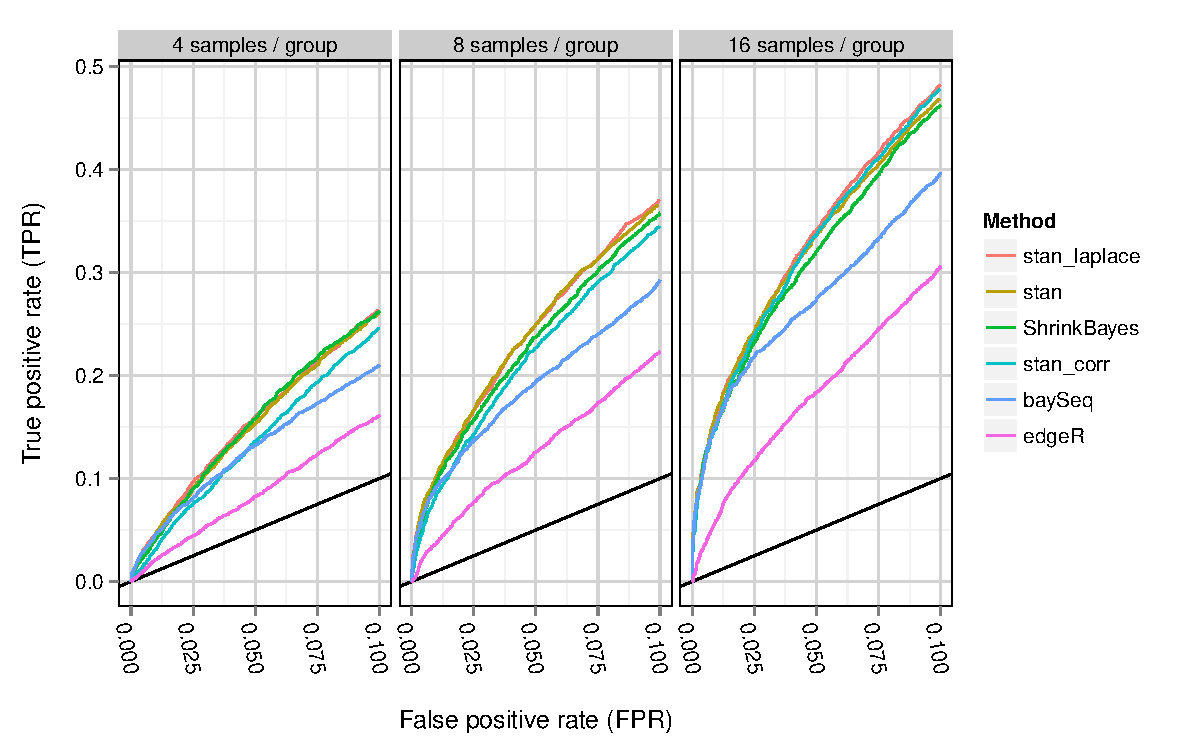
\includegraphics[width=0.8\textwidth]{exampleROC0_1}}
\caption{Example ROC curves for the first simulation}
\label{f:roc}
\end{figure}

\begin{figure}
\centerline{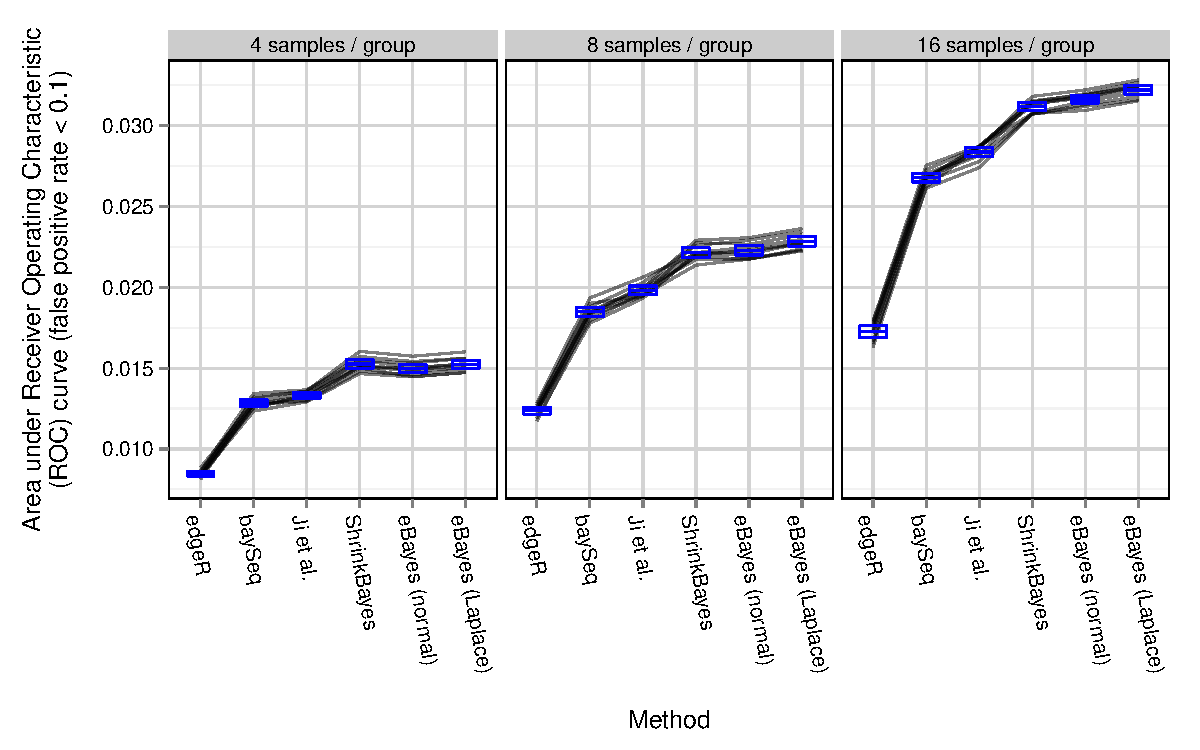
\includegraphics[width=0.8\textwidth]{auc-facet-TRUE}}
\caption{Area under the ROC curves (AUC) for 3 different sample sizes (facets) for the methods under comparison for false positive rates below 0.1. Each line is a different simulation while the blue box indicates mean AUC and its standard error across the simulations.}
\end{figure}

\section{Heterosis in corn ??}
\label{s:corn}

\section{Discussion}
\label{s:discuss}

Put your final comments here. 



\backmatter %  Please keep this command in your document in this position 



\section*{Acknowledgements}

The authors thank Andrew Lithio for help implementing our model in {\tt ShrinkBayes}.

%  If your paper refers to supplementary web material, then you MUST
%  include this section!!  See Instructions for Authors at the journal
%  website http://www.biometrics.tibs.org

\section*{Supplementary Materials}


\bibliography{jarad}
\bibliographystyle{biom}

\appendix

%  To get the journal style of heading for an appendix, mimic the following.

\section{}

The following sections provide Stan model code for performing the optimization and MCMC described in Section \ref{s:ebayes}. In these models, it is easier to construct the model using a single index, i.e. $y_i$, and then provide vectors that provide relevant quantities for this observation. These vectors include $g$ which indicates the gene, $v$ which indicates the variety, and $s$ which gives the sample index, i.e. a distinct identifier for the variety-replicate combation. 

\subsection{Optimization models}

The following two sections provide Stan model code for the optimization procedure, using the {\tt optimizing} function in RStan, either assuming independence or estimating a covariance amongst the location and (log) dispersion parameters. 

\subsubsection{All genes model}
\label{s:all_genes_model}

This section provides Stan model code for the model that assumes prior independence amongst the location and dispersion parameters. 

\begin{verbatim}
data{
  int N; //total # obs
  int G; // # genes
  int S; // # samples
  int<lower=0> y[N];
  int<lower=1,upper=G> g[N]; //obs -> gene
  int<lower=1,upper=3> t[N]; //obs -> genotype
  int<lower=1,upper=S> s[N]; //obs -> sample (genotype*rep)
  row_vector[3] X[3]; // mean structure (genotype)
}
parameters{
  matrix[3,G] B;         //phi, alpha, gamma by gene
  vector[G] lpsi;        //'dispersion'
  vector[S] c;           //lane sequencing depth
  real<lower=-20,upper=20> mu_phi;
  real<lower=-20,upper=20> mu_alpha;
  real<lower=-20,upper=20> mu_delta;
  real<lower=-20,upper=20> mu_psi;
  real<lower=0,upper = 20> sigma_phi;
  real<lower=0,upper = 20> sigma_alpha;
  real<lower=0,upper = 20> sigma_delta;
  real<lower=0,upper = 20> sigma_psi;
  real<lower=0,upper=5> sigma_c;
}

model{
  lpsi ~ normal(mu_psi,sigma_psi);
  B[1] ~ normal(mu_phi,sigma_phi);
  B[2] ~ normal(mu_alpha,sigma_alpha);
  B[3] ~ normal(mu_delta,sigma_delta);
  c ~ normal(0,sigma_c);
  for(n in 1:N){
    y[n] ~ neg_binomial_2_log(X[t[n]]*col(B,g[n]) + c[s[n]], 1 / exp(lpsi[g[n]]));
  }
  sigma_psi ~ cauchy(0,3);
  sigma_phi ~ cauchy(0,3);
  sigma_alpha ~ cauchy(0,3);
  sigma_delta ~ cauchy(0,3);
}
\end{verbatim}

\subsubsection{All genes model with covariance}
\label{s:all_genes_model_with_covariance}

This section provides Stan model code for the model that estimates the covariance structure amongst the location and (log) dispersion parameters. 

\begin{verbatim}
data{
  int N; //total # obs
  int G; // # genes
  int S; // # samples
  int<lower=0> y[N];
  int<lower=1,upper=G> g[N]; //obs -> gene
  int<lower=1,upper=3> t[N]; //obs -> genotype
  int<lower=1,upper=S> s[N]; //obs -> sample (genotype*rep)
  row_vector[4] X[3]; // mean structure (genotype)
}
parameters{
  vector[4] B[G];         //mu1, mu2, mu3, lpsi by gene
  vector[S] c;            //lane sequencing depth
  vector<lower=-20,upper=20>[4] mu;
  cov_matrix[4] Sigma;
  real<lower=0,upper=5> sigma_c;
}

model{
  vector[4] x;
  for(i in 1:G){
    B[i] ~ multi_normal(mu, Sigma);
  }
  c ~ normal(0,sigma_c);
  for(n in 1:N){
    y[n] ~ neg_binomial_2_log(X[t[n]]*B[g[n]] + c[s[n]], 1 / exp(B[g[n],4]));
  }
  x <-rep_vector(1,4);
  Sigma ~ inv_wishart(5.0,diag_matrix(x));
}
\end{verbatim}

\subsection{Models for MCMC}

As described in Section \ref{s:ebayes}, conditional on the hyperparameters inference on the gene-specific parameters can be performed independently and in parallel. This section provides Stan model code for single-gene models either assuming independence or with a covariance structure amongst the location and (log) dispersion parameter. These model files are used in conjunction with the {\tt sampling} function in RStan. 

\subsubsection{Single-gene model assuming independence}
\label{s:single_gene_model}

This section provides Stan model code for the single-gene model where independence is assumed amongst the location and (log) dispersion parameters.

\begin{verbatim}
data{
  int N; //total # obs
  int S; // # samples
  int<lower=0> y[N];
  int<lower=1,upper=3> t[N]; //obs -> genotype
  int<lower=1,upper=S> s[N]; //obs -> sample (genotype*rep)
  row_vector[3] X[3]; // mean structure (genotype)
  real<lower=-20,upper=20> mu_phi;
  real<lower=-20,upper=20> mu_alpha;
  real<lower=-20,upper=20> mu_delta;
  real<lower=-20,upper=20> mu_psi;
  real<lower=0,upper = 20> sigma_phi;
  real<lower=0,upper = 20> sigma_alpha;
  real<lower=0,upper = 20> sigma_delta;
  real<lower=0,upper = 20> sigma_psi;
  vector[S] c;            //lane sequencing depth
}
transformed data{
  vector[3] Mu;
  cov_matrix[3] Sigma;
  Mu[1] <- mu_phi;
  Mu[2] <- mu_alpha;
  Mu[3] <- mu_delta;
  Sigma[1,2] <- 0;
  Sigma[2,1] <- 0;
  Sigma[1,3] <- 0;
  Sigma[3,1] <- 0;
  Sigma[2,3] <- 0;
  Sigma[3,2] <- 0;
  Sigma[1,1] <- square(sigma_phi);
  Sigma[2,2] <- square(sigma_alpha);
  Sigma[3,3] <- square(sigma_delta);
}
parameters{
  vector[3] B;         //phi, alpha, gamma by gene
  real lpsi;       //'dispersion'
}

model{
  lpsi ~ normal(mu_psi,sigma_psi);
  B    ~ multi_normal(Mu,Sigma);
  for(n in 1:N){
    y[n] ~ neg_binomial_2_log(X[t[n]]*B + c[s[n]], 1 / exp(lpsi));
  }
}
\end{verbatim}

\subsection{Single-gene model with covariance}
\label{s:single_gene_model_with_covariance}

This section provides Stan model code for the single-gene model where a covariance amongst the location and (log) dispersion parameters is used.

\begin{verbatim}
data{
  int N; //total # obs
  int S; // # samples
  int<lower=0> y[N];
  int<lower=1,upper=3> t[N]; //obs -> genotype
  int<lower=1,upper=S> s[N]; //obs -> sample (genotype*rep)
  row_vector[4] X[3]; // mean structure (genotype)
  vector[S] c;            //lane sequencing depth
  vector<lower=-20,upper=20>[4] mu;
  real<lower=0> sigma_phi;
  real<lower=0> sigma_alpha;
  real<lower=0> sigma_delta;
  real<lower=0> sigma_psi;
  real cor_12;
  real cor_13;
  real cor_14;
  real cor_23;
  real cor_24;
  real cor_34;
  real<lower=0,upper=5> sigma_c;
}
transformed data{
  cov_matrix[4] Sigma;
  Sigma[1,2] <- cor_12;
  Sigma[2,1] <- cor_12;
  Sigma[1,3] <- cor_13;
  Sigma[3,1] <- cor_13;
  Sigma[1,4] <- cor_14;
  Sigma[4,1] <- cor_14;
  Sigma[2,3] <- cor_23;
  Sigma[3,2] <- cor_23;
  Sigma[2,4] <- cor_24;
  Sigma[4,2] <- cor_24;
  Sigma[3,4] <- cor_34;
  Sigma[4,3] <- cor_34;
  Sigma[1,1] <- sigma_phi;
  Sigma[2,2] <- sigma_alpha;
  Sigma[3,3] <- sigma_alpha;
  Sigma[4,4] <- sigma_psi;
}
parameters{
  vector[4] B;         //phi, alpha, gamma by gene
}

model{
  B    ~ multi_normal(mu,Sigma);
  for(n in 1:N){
    y[n] ~ neg_binomial_2_log(X[t[n]]*B + c[s[n]], 1 / exp(B[4]));
  }
}
\end{verbatim}

\label{lastpage}

\end{document}
